\subsection{Huffman Coding}

Er en komprimeringsalgoritme, som forsøger at bruge så få bits som muligt. Den er også \textit{lossless}.\\

Ser på de enkelte pixel værdier og antallet af deres forekomster.\\

Eksempelvis hvis en pixel værdien 87 fylder 30\% af billeder og hver forekomst af denne repræsenteres med 8 bit. Man kan da repræsentere denne værdi kortere ved at kalde værdien 01 (binært), hvilket kun fylder 2 bit.

\subsubsection{Huffman Eksempel}

Figur~\ref{fig:hoffman-coding-1} og \ref{fig:hoffman-coding-2} viser hvordan Huffman coding foretages.

\begin{figure}[H]
	\centering
	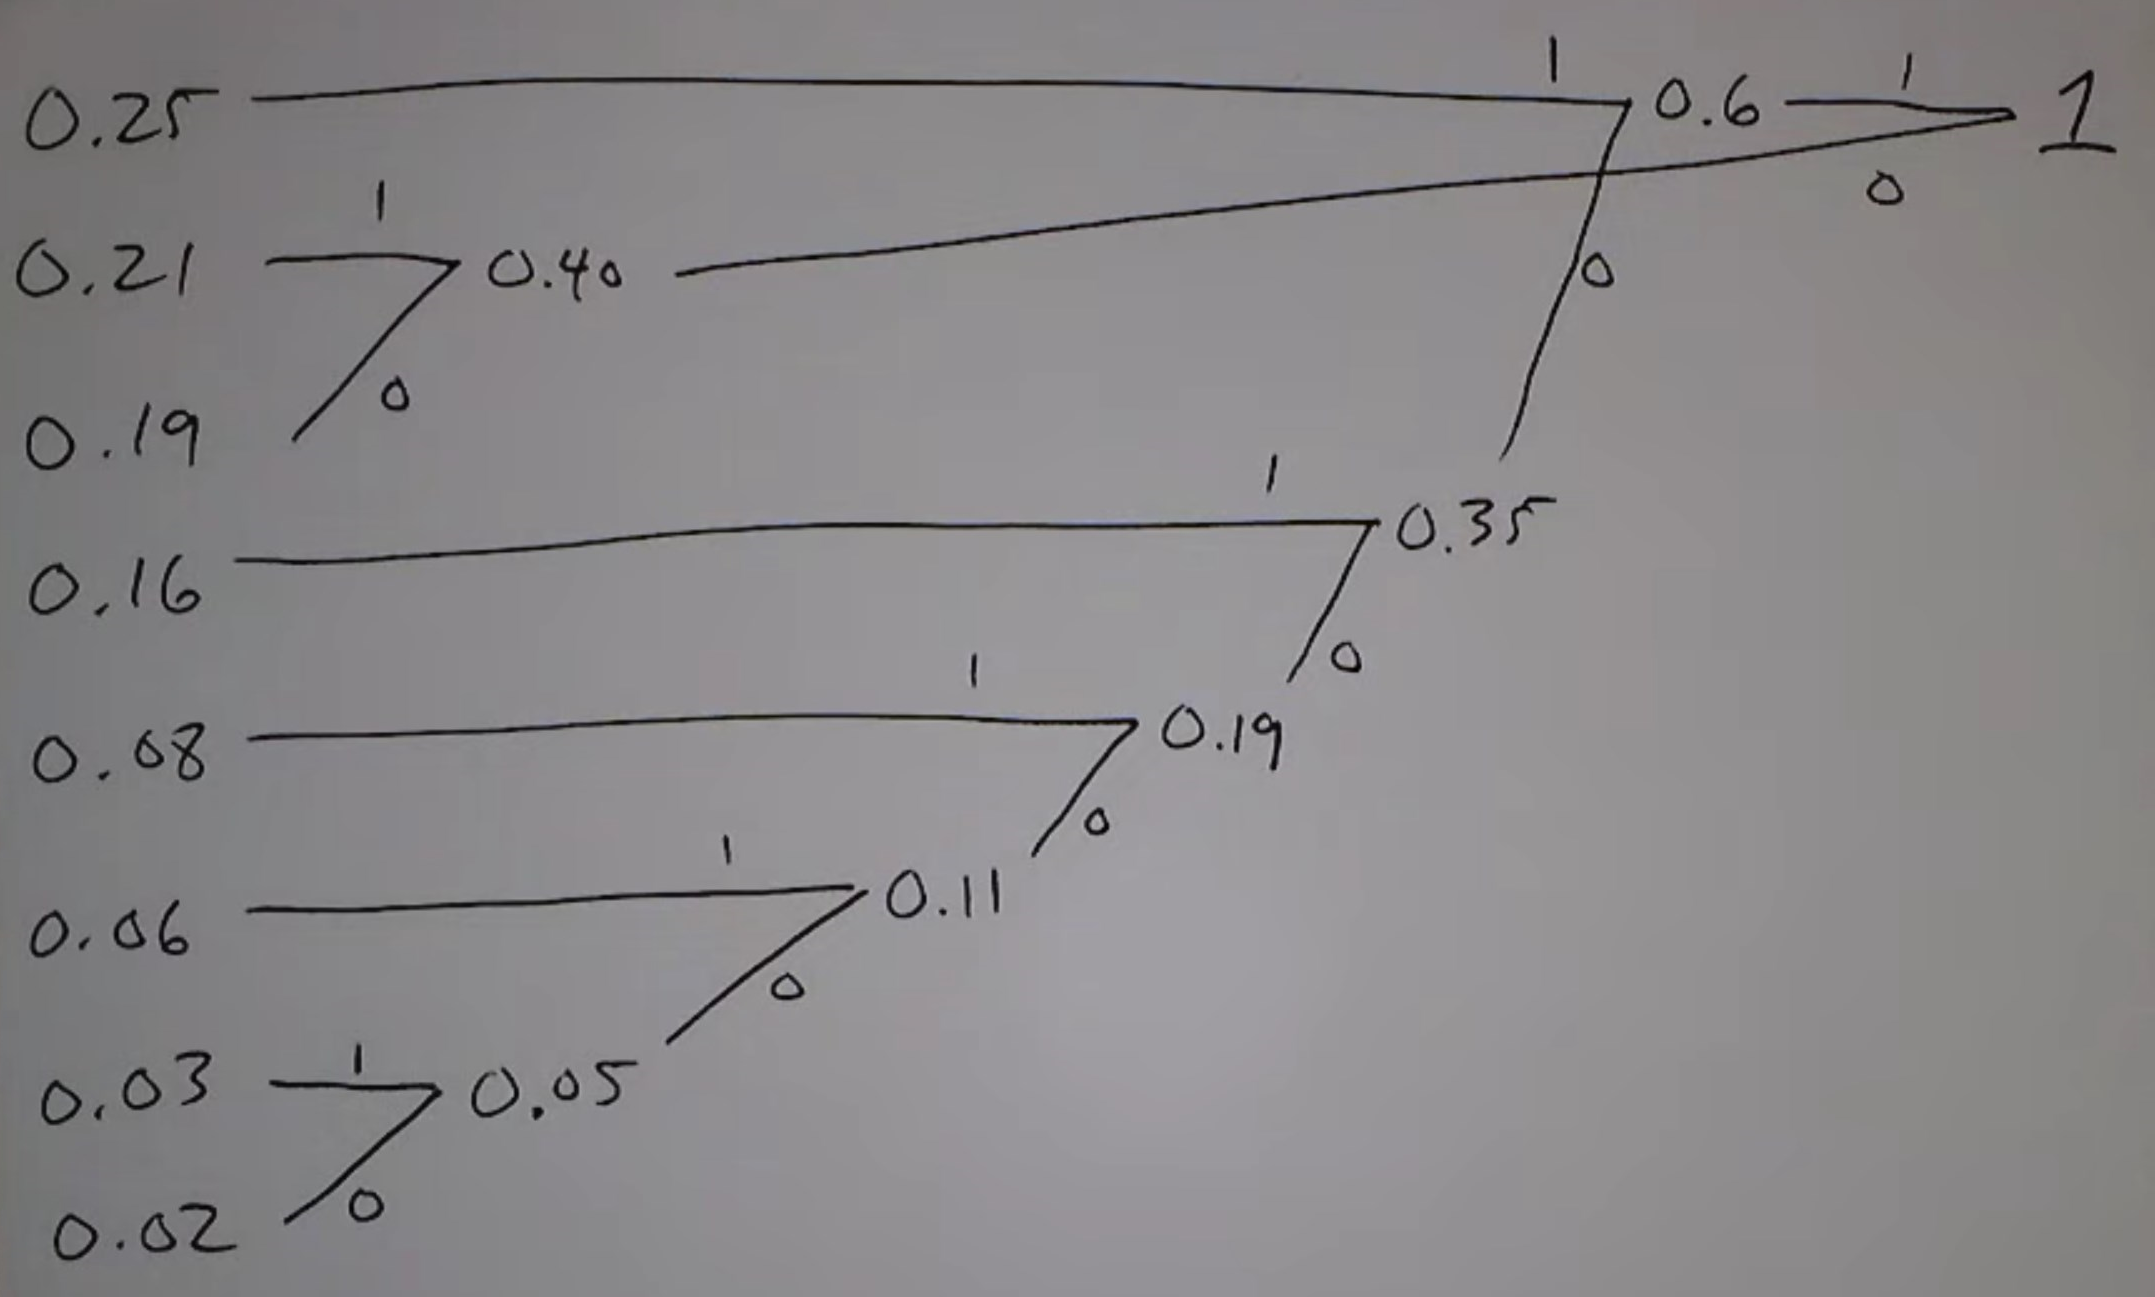
\includegraphics[width=0.8\linewidth]{figs/spm08/hoffman-coding-1}
	\caption{Forklaring af Huffman coding.}
	\label{fig:hoffman-coding-1}
\end{figure}

\begin{figure}[H]
	\centering
	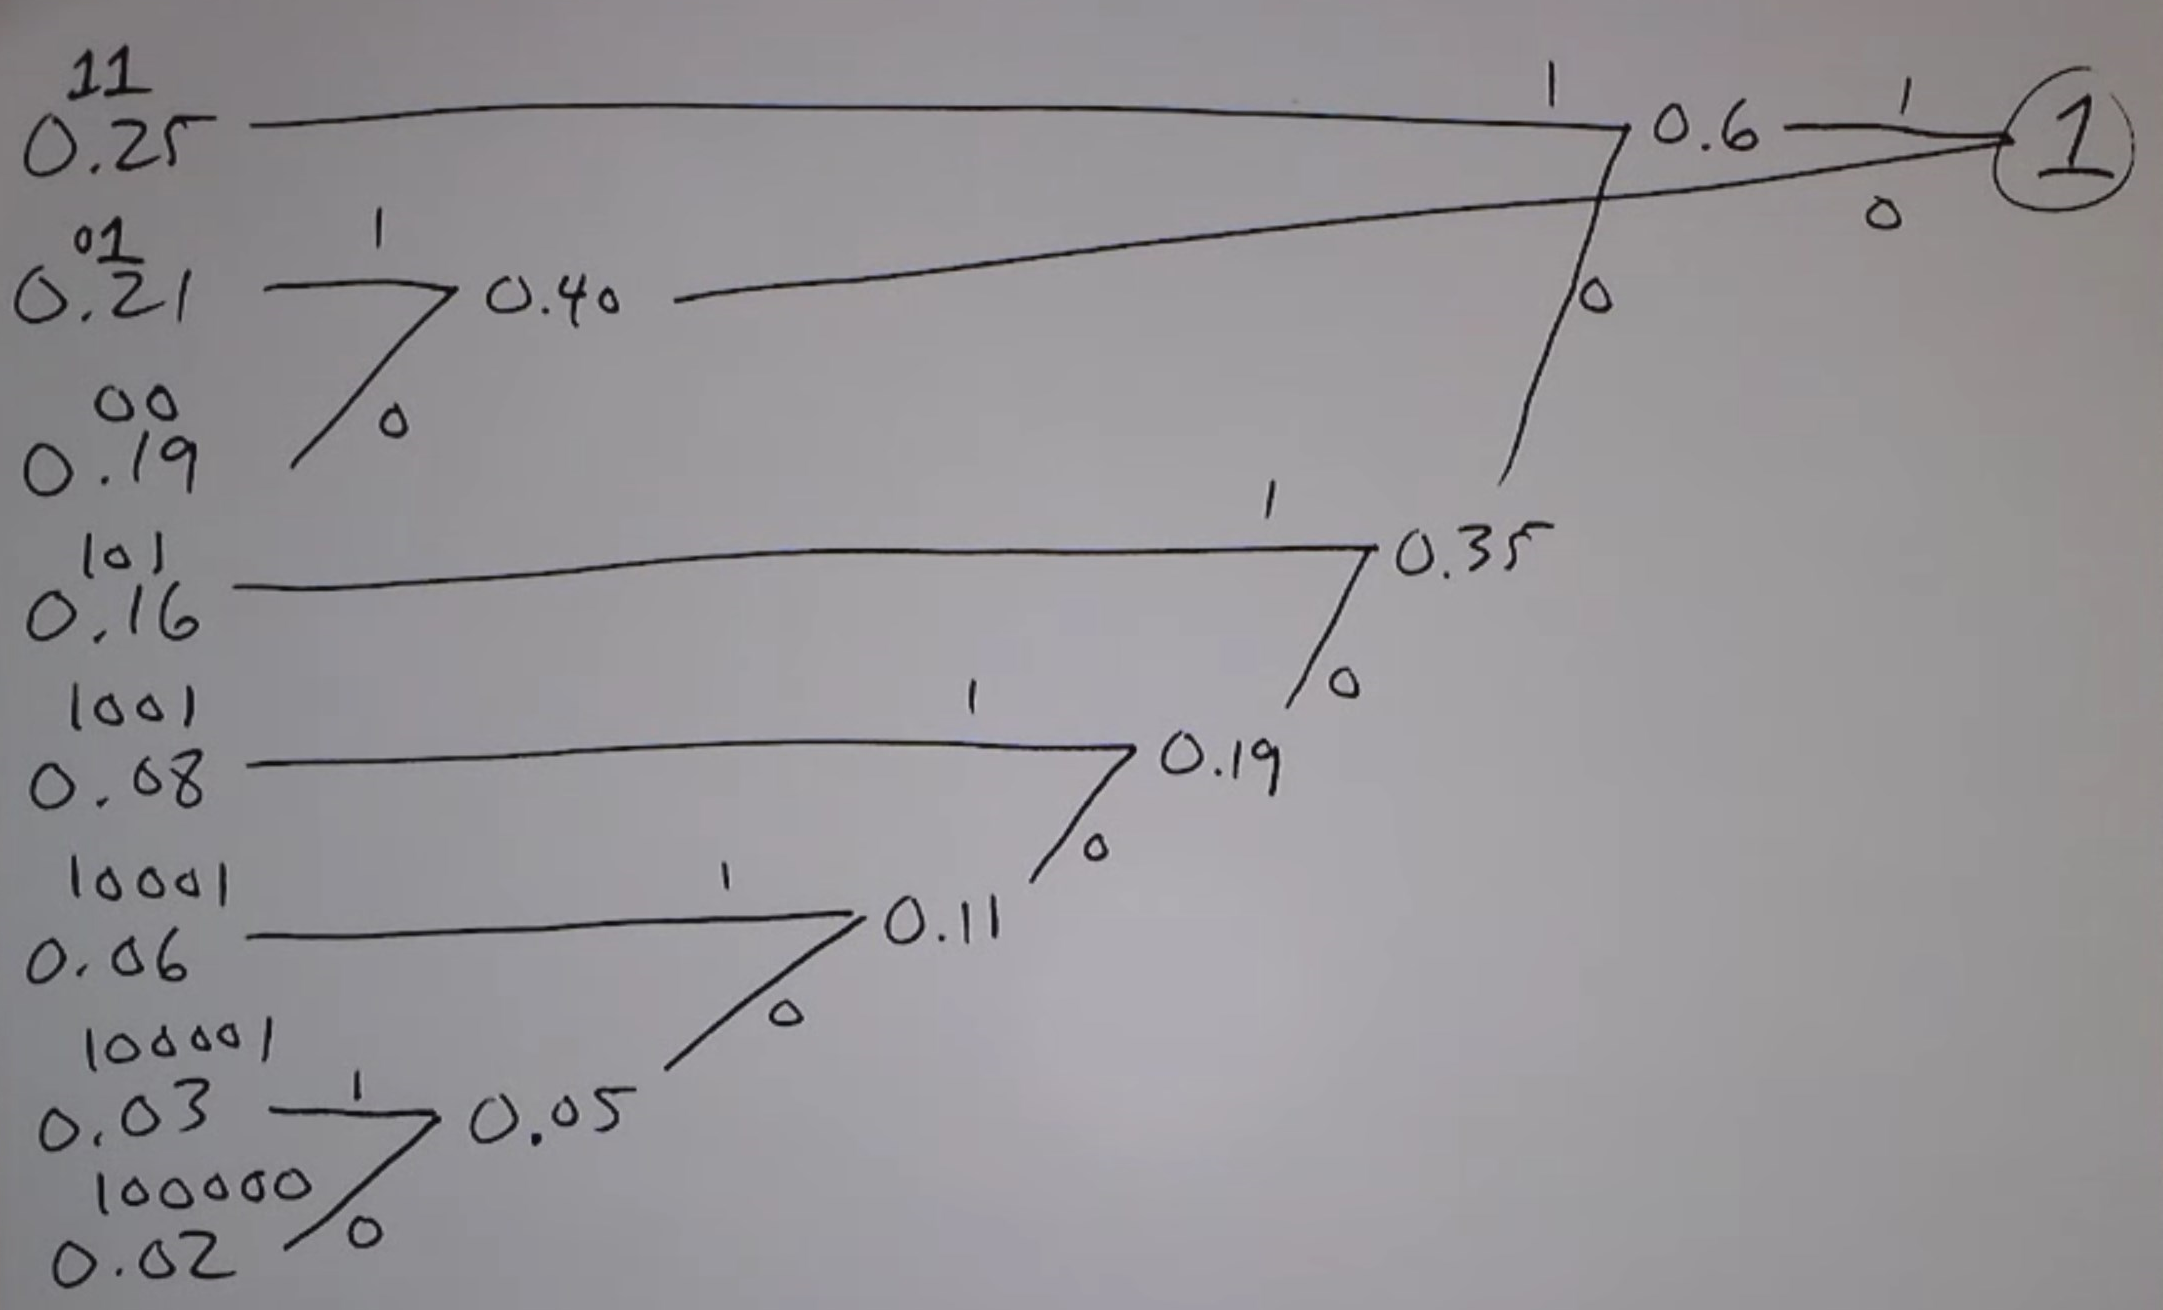
\includegraphics[width=0.8\linewidth]{figs/spm08/hoffman-coding-2}
	\caption{Forklaring af Huffman coding med binære tal.}
	\label{fig:hoffman-coding-2}
\end{figure}

Som en bonus er Huffman coding også en \textit{Prefix code}. Hvilket vil sige: at ingen kode er prefix til en anden kode. 

På grund af denne smarte egenskab kan de dekode strengen direkte (når vi møder hver codeword) og vi behøver derfor ikke læse mere end én kode frem for at kunne dekode noget. Vist på Figur~\ref{fig:prefix}.\\

\begin{figure}[H]
	\centering
	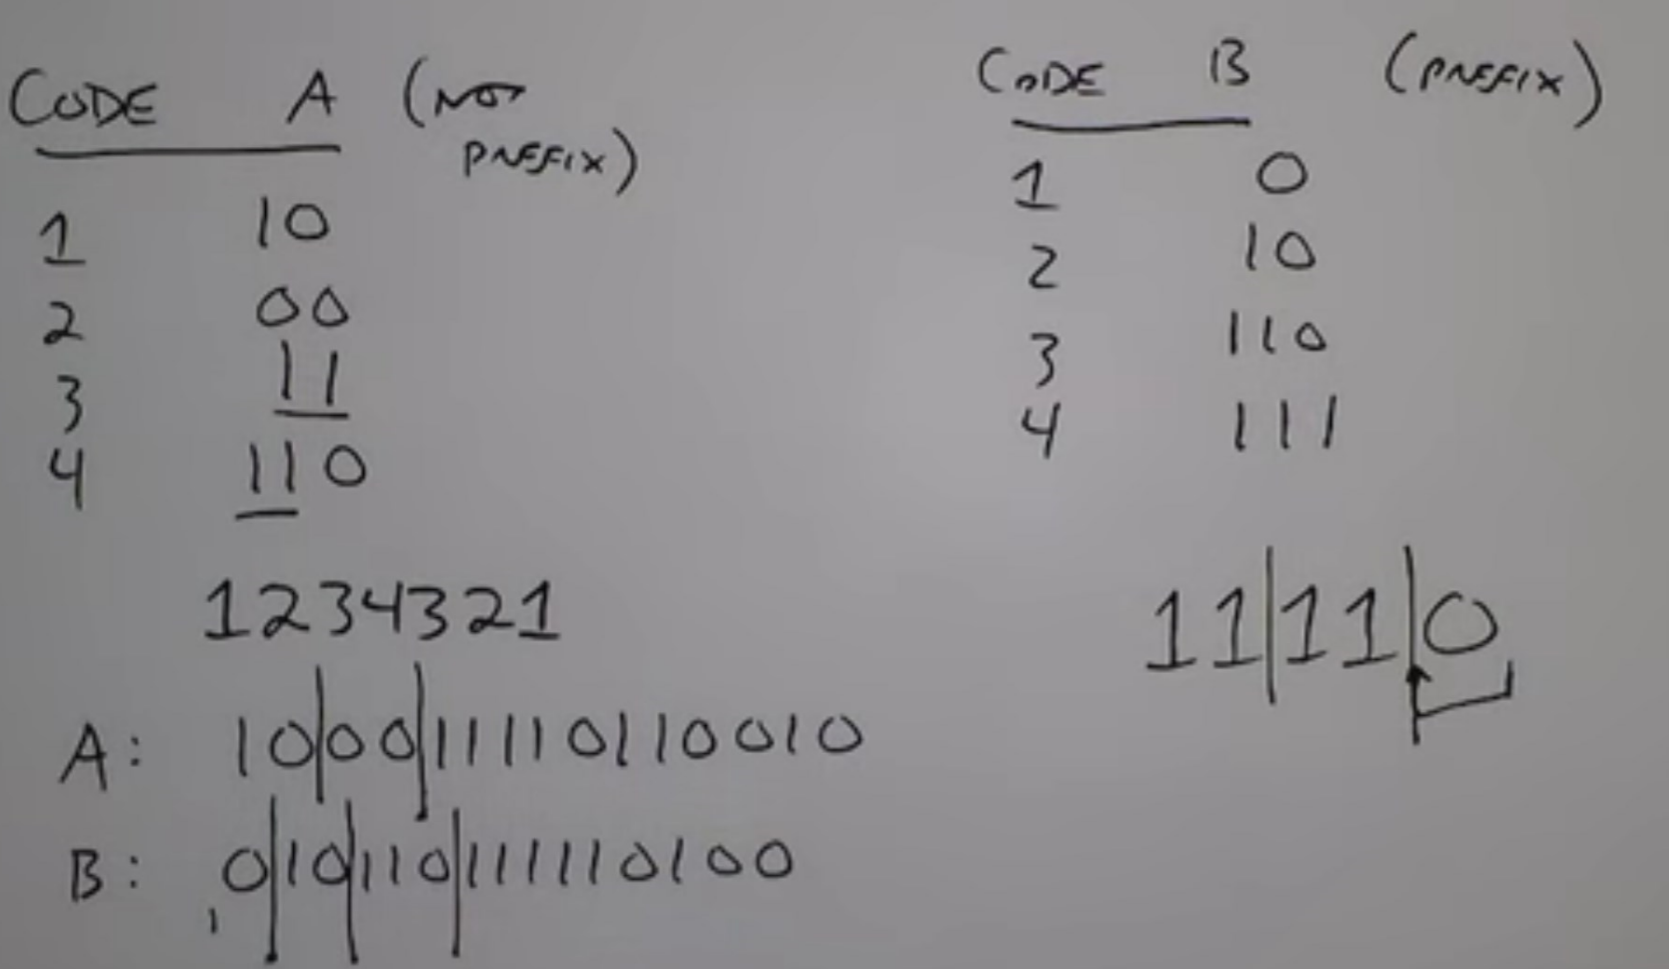
\includegraphics[width=0.9\linewidth]{figs/spm08/prefix}
	\caption{Illustration af prefix code betydningen.}
	\label{fig:prefix}
\end{figure}

